% !TeX program = xelatex
% !BIB program = biber
% !TeX TXS-program:bibliography = txs:///biber
\documentclass[10pt,a4paper]{article}
\usepackage[utf8]{inputenc}
\usepackage[T1]{fontenc}
\usepackage{amsmath}
\usepackage{amssymb}
\usepackage{graphicx}
\usepackage{color,soul}
\usepackage{easyReview}
\usepackage{booktabs}
\usepackage{multirow}
\usepackage[section]{placeins}
\usepackage[hidelinks]{hyperref}
\usepackage[backend=biber, style=numeric, citestyle=numeric-comp, sorting=none, hyperref=true, maxnames=20]{biblatex}
\usepackage[nottoc]{tocbibind} % la opcion nottoc hace que el indice no aparezca
% en la tabla de contenidos
\usepackage[a4paper, margin=30mm]{geometry}
\usepackage{authblk}
\usepackage{lineno}
\usepackage{float}
\usepackage{indentfirst}
\usepackage[none]{hyphenat}
\usepackage{acronym}
\usepackage{nomencl}
\usepackage{lineno}
\usepackage[breakable]{tcolorbox}

\usepackage[spanish]{babel} % para que no diga "chapter", y diga "capítulo"
\usepackage{pdfpages} % Para insertar PDFs
\usepackage{tabularx}
\usepackage{csquotes}
\usepackage{titling}

\addto\captionsspanish{\renewcommand{\tablename}{Tabla}}

% \linenumbers

%%% carpeta de figuras %%%%%%
\graphicspath{{figs/}}

\addbibresource{bibliografia_2026.bib}

%%%%%%%% algunas cosas para renderizar mejor las ecuaciones %%%%%%%%%%%%
\DeclareMathSizes{10}{9}{7}{5}

% overline con mas espacio entre letras y barra
\newcommand*\oline[1]{%
	\vbox{%
		\hrule height 0.5pt%                  % Line above with certain width
		\kern0.4ex%                          % Distance between line and content
		\hbox{%
			\kern-0.1em%                        % Distance between content and left side of box, negative values for lines shorter than content
			\ifmmode#1\else\ensuremath{#1}\fi%  % The content, typeset in dependence of mode
			\kern-0.1em%                        % Distance between content and left side of box, negative values for lines shorter than content
		}% end of hbox
	}% end of vbox
}

\newcommand{\norma}[1]{\left\|#1\right\|}
\newcommand{\abector}[2]{\oline{#1#2}}
\newcommand{\pdv}[2]{\dfrac{\partial #1}{\partial #2}}

%\linenumbers

\linespread{1.5} % espacio de interlineado
% Set the space after paragraphs
\setlength{\parskip}{1em} % Adjust the length as needed

%\pretitle{\begin{center}\Large\bfseries}
%	\posttitle{\end{center}}
%\preauthor{}
%\postauthor{}
%\predate{}
%\postdate{}
%
%\title{Momentum CSIC\\
%	 \small Tecnología de imagen multi-modal para investigación pre-clínica (TIMPRE)\\
%	 \large Memoria anual 2026}
%	 \author{\centering Guillermo G. Cosarinsky Markman}
%\date{}

\title{
	\textbf{Momentum CSIC} \\
	Tecnología de imagen multi-modal para investigación pre-clínica (TIMPRE) \\
	Memoria anual 2026
}
\author{Guillermo G. Cosarinsky Markman}
\date{}

%%%%%%%%%%%%%%%%%%%%%%%%%%%%%%%%%%%%%%%%%%%%%%%%%%%%%%%%%%%%%%%%%%%%%%%%%%%%%%%%%%%%%%%%%%%%%


\newcommand{\pendiente}[1]{\par\begingroup\raggedright\noindent\textcolor{gray}{\textit{[Pendiente: #1]}}\par\endgroup}

\begin{document}
\maketitle
\thispagestyle{empty}
\vspace{5cm}
\begin{center}
	
\includegraphics[width=0.9\textwidth]{logos_todos.png}
\end{center}

\newpage

\tableofcontents
\clearpage

% PLANTILLA DE TRABAJO
% Cuerpo orientativo: 10--12 paginas una vez completado, sin referencias ni anexos.
% Mantener una redaccion sintetica centrada en actividades y resultados documentados.
% Sustituir las llamadas a \pendiente por texto final y eliminarlas al cerrar la memoria.
% No incorporar analisis nuevos; resumir el TFM y el articulo de Tecniacustica.

\section{Introducción y objetivos del año}\label{sec:intro}
La presente memoria resume las actividades realizadas durante 2026 en el marco del proyecto Tecnología de imagen multi-modal para investigación pre-clínica (TIMPRE), financiado por el programa Momentum CSIC.

Durante 2026 se dio continuidad al estudio de la técnica de formación de imagen \textit{Null Subtraction Imaging} (NSI)~\cite{Agarwal2019}, iniciado en la anualidad anterior~\cite{CosarinskyMemoria2025}. Esta técnica combina imágenes obtenidas con distintas apodizaciones de recepción, es decir, con diferentes distribuciones de pesos aplicados a las señales de los elementos del array antes de sumarlas para formar cada imagen. La elección de estos pesos influye en el equilibrio entre la resolución espacial y la supresión de lóbulos laterales. Durante el desarrollo del trabajo en 2025 se identificaron limitaciones asociadas al recorte de la apertura de recepción en las proximidades de los bordes del array. Estas observaciones motivaron la investigación de nuevas apodizaciones diseñadas mediante representaciones neuronales implícitas (\textit{Implicit Neural Representations}, INR)~\cite{Molaei2023}. Estas representaciones utilizan una red neuronal para describir una función continua a partir de sus coordenadas de entrada; en este caso, la red recibe las coordenadas del punto de la imagen y del elemento del array y devuelve el peso de apodización correspondiente. Esto permite adaptar los pesos de recepción a la geometría de cada punto de la imagen. Como primer paso, se desarrolló un Trabajo de Fin de Máster\footnote{Este trabajo corresponde al Máster de Formación Permanente en Inteligencia Artificial Aplicada de la Universidad Europea, iniciado en 2025 como parte de las actividades formativas del programa Momentum CSIC. La memoria completa del TFM se adjunta en el Anexo~\ref{anexo:tfm}.} centrado en la optimización de una única apodización mediante una INR~\cite{CosarinskyTFM2026}. Posteriormente, esta línea se amplió al diseño de múltiples apodizaciones y a la combinación de las envolventes de las imágenes resultantes mediante una segunda red neuronal, denominada \textit{mixer}, dando lugar al trabajo presentado en Tecniacústica 2026~\cite{CosarinskyTecniacustica2026}.

En cuanto a la formación en competencias digitales, durante 2026 cursé los últimos módulos del Máster de Formación Permanente en Inteligencia Artificial Aplicada de la Universidad Europea y realicé el Trabajo de Fin de Máster. Esta formación me permitió profundizar en el diseño, entrenamiento y evaluación de modelos de aprendizaje automático y aplicar estos conocimientos al desarrollo de apodizaciones para imagen ultrasónica.

Con el propósito de ampliar la aplicación de estas competencias en inteligencia artificial a otros problemas de imagen ultrasónica, inicié una estancia de investigación en la Universidad Complutense de Madrid (UCM), en el Departamento de Estructura de la Materia, Física Térmica y Electrónica, bajo la supervisión del profesor Joaquín López Herraiz. La estancia tiene como objetivo investigar métodos de IA para el guiado de ecocardiografías, incorporando así una nueva línea de trabajo centrada en la asistencia durante la adquisición de imágenes. El periodo previsto para la estancia comprende del 16 de septiembre al 11 de diciembre de 2026.

Como complemento a estas actividades de formación e investigación, participé en la organización del simposio SABIA 2026 (\textit{Symposium on Advanced Biomedical Instrumentation \& Applications}) y fui \textit{chairman} en una de sus sesiones, contribuyendo al intercambio científico en el ámbito de la instrumentación biomédica.


\section{Desarrollo de métodos de beamforming con IA}\label{sec:beamforming}
% Extension orientativa del conjunto de la seccion: 4--5 paginas.

El método de retardo y suma (\textit{Delay-and-Sum}, DAS) forma cada punto de la imagen alineando temporalmente las señales recibidas por los elementos del array según los tiempos de propagación. Las señales alineadas se ponderan mediante la apodización de recepción y se suman para obtener el valor de imagen~\cite{Perrot2021}.

Como punto de partida de esta línea de trabajo, se retomó el método NSI estudiado durante 2025~\cite{CosarinskyMemoria2025}. En su formulación para arrays lineales, NSI combina de forma no lineal las envolventes de tres imágenes conformadas mediante DAS con distintas apodizaciones de recepción~\cite{Agarwal2019}. Utilizando la letra $a$ para las apodizaciones, de forma coherente con el TFM, estas se denominan $a_{zm}$, $a_{dc1}$ y $a_{dc2}$ y se definen, para una subapertura de recepción de $N$ elementos con $N$ par, como:
\begin{align}
  a_{zm}[n] &= \begin{cases}
    -1, & 0\leq n<N/2,\\
    +1, & N/2\leq n<N,
  \end{cases}\label{eq:nsi_apod_zm}\\
  a_{dc1}[n] &= a_{zm}[n]+dc\,a_u[n],\\
  a_{dc2}[n] &= -a_{zm}[n]+dc\,a_u[n],
\end{align}
Aquí, $N$ representa el número de elementos de la subapertura activa y puede ser menor que el número total de elementos del array físico; $n$ es el índice local dentro de esa subapertura. La selección de elementos puede depender de la posición del píxel y de la profundidad. Por su parte, $a_u[n]=1$ es la apodización uniforme sobre la subapertura y $dc$ es un pequeño desplazamiento positivo. La distribución $a_{zm}$ tiene media cero: bajo condiciones de simetría, las contribuciones de ambas mitades de la apertura se cancelan en la dirección de enfoque y generan un nulo central en la respuesta lateral.

Sean $I_{zm}(P)$, $I_{dc1}(P)$ e $I_{dc2}(P)$ las imágenes DAS complejas obtenidas con estas apodizaciones en el punto $P$, cuyas envolventes son $|I_{zm}(P)|$, $|I_{dc1}(P)|$ e $|I_{dc2}(P)|$, respectivamente. La imagen NSI se calcula mediante:
\begin{equation}
  I_{\mathrm{NSI}}(P)=\frac{1}{2}\left(|I_{dc1}(P)|+|I_{dc2}(P)|\right)-|I_{zm}(P)|.
  \label{eq:nsi_combinacion}
\end{equation}
La sustracción de la envolvente con nulo central permite obtener una respuesta lateral más estrecha que la de DAS con apodización uniforme, en las condiciones estudiadas en la bibliografía citada.


La Figura~\ref{fig:nsi_apodizaciones} muestra las tres apodizaciones descritas para una subapertura lineal simétrica de 64 elementos.

\begin{figure}[htbp]
  \centering
  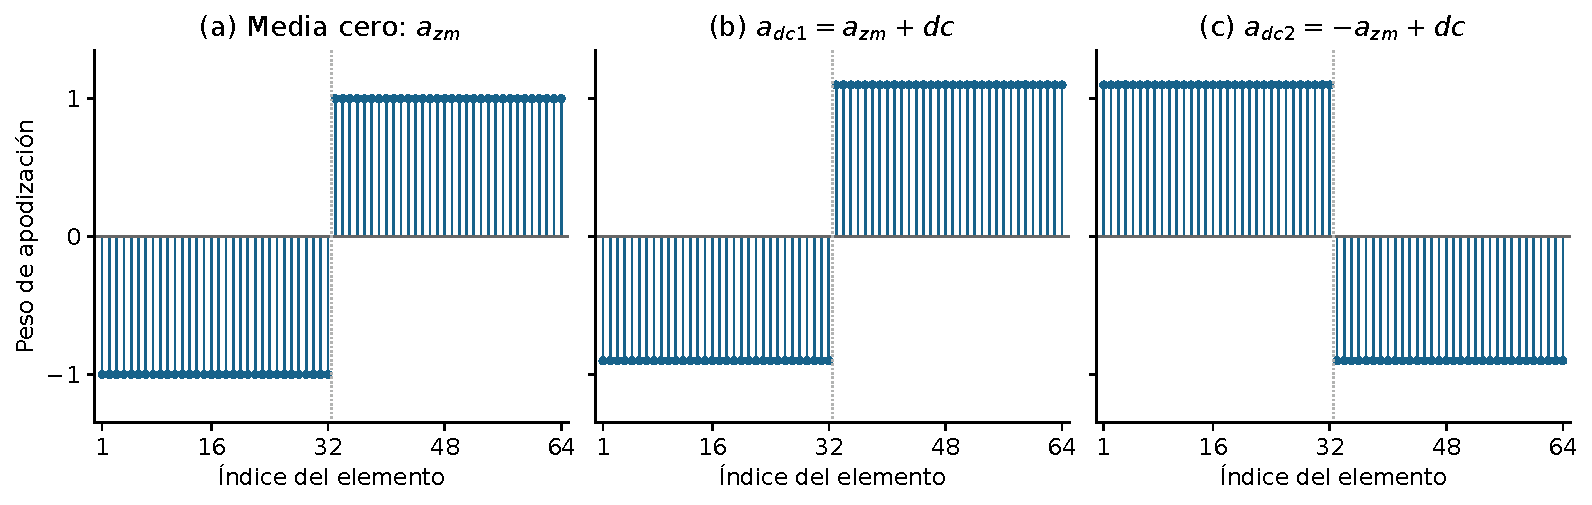
\includegraphics[width=\textwidth]{nsi_apodizaciones_lineales.pdf}
  \caption{Apodizaciones de recepción de NSI para una subapertura lineal simétrica de 64 elementos: (a) distribución de media cero $a_{zm}$, con pesos $-1$ y $+1$ en las dos mitades de la apertura; (b) $a_{dc1}=a_{zm}+dc$; (c) $a_{dc2}=-a_{zm}+dc$, con $dc=0.1$. Las imágenes correspondientes se denotan $I_{zm}$, $I_{dc1}$ e $I_{dc2}$ y se combinan según la Ecuación~\eqref{eq:nsi_combinacion}.}
  \label{fig:nsi_apodizaciones}
\end{figure}

Para ilustrar esta combinación, se calcularon los perfiles laterales de campo lejano de las tres apodizaciones, con una subapertura simétrica de $N=64$ elementos, $dc=0.1$ y separación entre elementos $d=2\lambda$. Se denomina $B_i(\theta)$ a la respuesta compleja asociada a cada apodización $a_i$. La Figura~\ref{fig:nsi_perfiles_componentes} muestra sus magnitudes y un detalle del nulo central. En este modelo simétrico, $|B_{dc1}|$ y $|B_{dc2}|$ coinciden. La Figura~\ref{fig:nsi_perfil_final} presenta la combinación de estas magnitudes según la Ecuación~\eqref{eq:nsi_combinacion}, comparada con el perfil de la apodización uniforme. Los gráficos muestran una ventana angular alrededor de la dirección de enfoque y describen la respuesta ideal del modelo.

\begin{figure}[htbp]
  \centering
  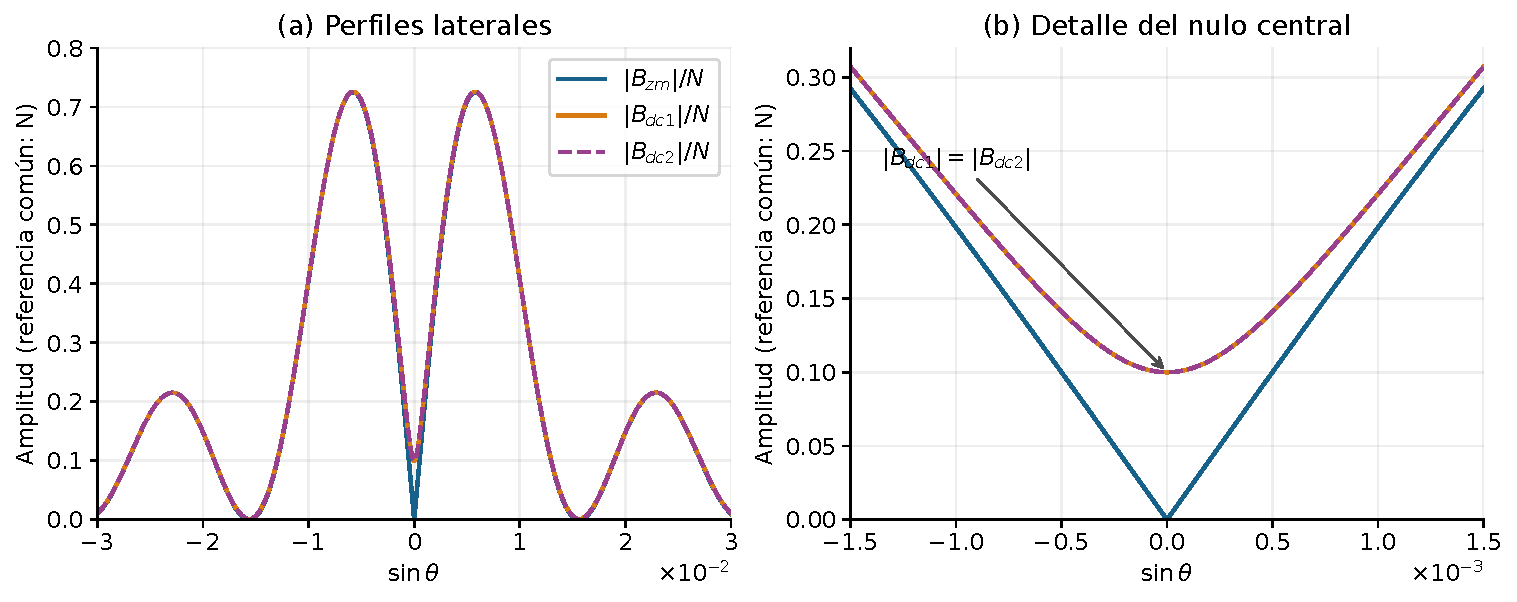
\includegraphics[width=\textwidth]{nsi_perfiles_componentes.pdf}
  \caption{Magnitudes de los perfiles laterales asociados a $a_{zm}$, $a_{dc1}$ y $a_{dc2}$: (a) vista general y (b) detalle del nulo central. Se utiliza una referencia común $N$ para conservar las amplitudes relativas que intervienen en la sustracción. Las curvas $|B_{dc1}|$ y $|B_{dc2}|$ se superponen y se distinguen por el estilo de línea. Parámetros: subapertura de $N=64$ elementos, $dc=0.1$ y $d=2\lambda$.}
  \label{fig:nsi_perfiles_componentes}
\end{figure}

\begin{figure}[htbp]
  \centering
  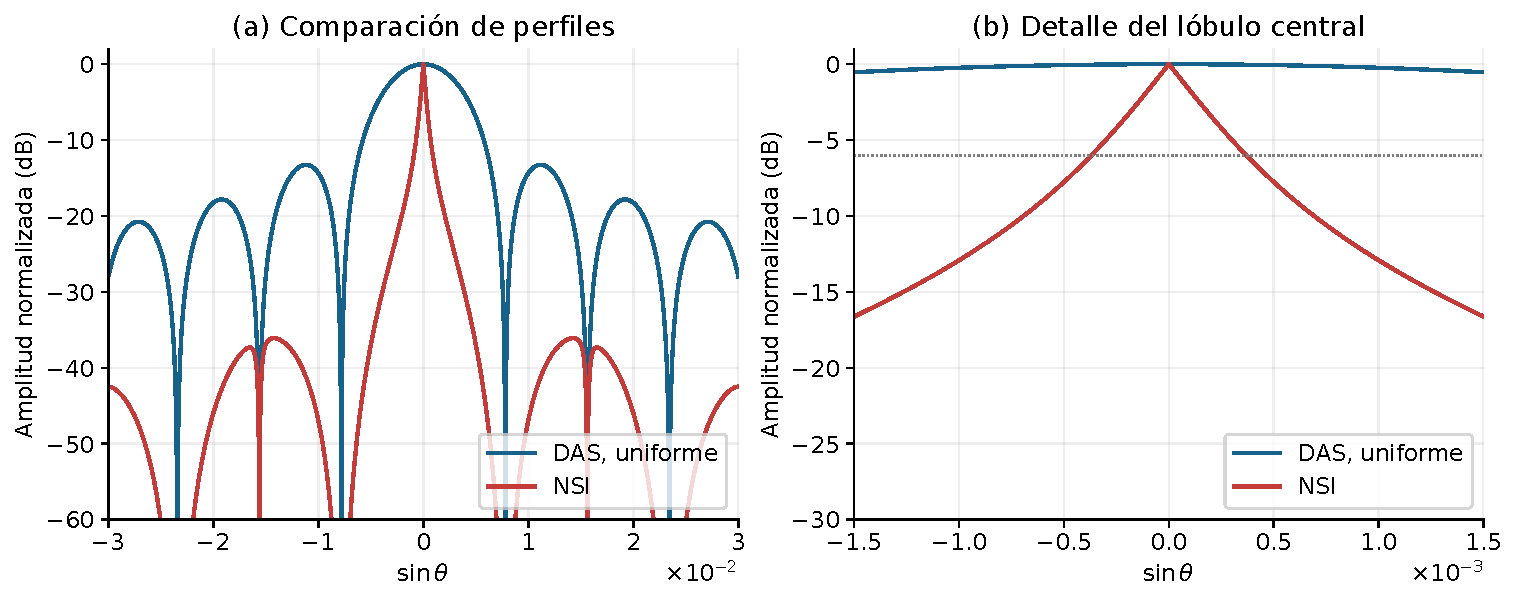
\includegraphics[width=\textwidth]{nsi_perfil_final_uniforme.pdf}
  \caption{Perfil lateral de la combinación NSI frente a DAS con apodización uniforme: (a) vista general y (b) detalle del lóbulo central. La combinación NSI se calcula con las amplitudes originales, antes de normalizar. Cada perfil final se normaliza por su propio máximo y se expresa como $20\log_{10}$ de la amplitud relativa. La línea horizontal discontinua señala $-6$~dB. Parámetros: subapertura de $N=64$ elementos, $dc=0.1$ y $d=2\lambda$.}
  \label{fig:nsi_perfil_final}
\end{figure}
\FloatBarrier


El funcionamiento de NSI depende del equilibrio entre los pesos positivos y negativos de la apertura. Al centrar lateralmente la subapertura de recepción en el punto de imagen, esta puede superar los límites físicos del array y quedar recortada. En estas condiciones, ambas regiones pueden quedar desequilibradas y alterar la cancelación esperada. Esta limitación, identificada durante el trabajo previo con NSI, motivó la búsqueda de nuevas apodizaciones que tuvieran en cuenta la geometría entre el punto de imagen y los elementos disponibles de la apertura.

Para explorar esta posibilidad, se planteó el diseño de apodizaciones como un problema de optimización mediante aprendizaje automático, utilizando una INR para representar los pesos de recepción en función de las coordenadas del punto de imagen y del elemento del array. Como primer paso, el TFM abordó el aprendizaje de una única apodización aplicada a DAS; posteriormente, el trabajo se amplió al aprendizaje de múltiples apodizaciones y su combinación mediante un \textit{mixer}. Estos desarrollos constituyen una base para investigar alternativas a las distribuciones prefijadas de NSI.

\subsection{Diseño de apodizaciones mediante INR}\label{sec:tfm}
Esta subsección presenta una síntesis del Trabajo de Fin de Máster~\cite{CosarinskyTFM2026}, centrada en el enfoque desarrollado y sus principales resultados. Los detalles técnicos, las definiciones completas y la descripción de los procedimientos de entrenamiento y evaluación pueden consultarse en la memoria del TFM incluida en el Anexo~\ref{anexo:tfm}.

Como antecedente directo, Delaunay et al.~\cite{Delaunay2025} propusieron una INR para aprender pesos complejos de apodización de recepción en ecocardiografía intracardíaca con ondas divergentes. Su red recibe las coordenadas del píxel y el ángulo de emisión, utiliza una codificación posicional y devuelve un vector de pesos para los canales de recepción. El entrenamiento emplea imágenes compuestas con 26 emisiones como referencia para mejorar reconstrucciones obtenidas con tres emisiones. Este trabajo constituye un ejemplo de integración de una representación neuronal continua en el proceso de conformación de imagen.

En el TFM~\cite{CosarinskyTFM2026} se estudió una formulación basada explícitamente en la geometría entre el píxel y cada elemento del array, aplicada a imagen con ondas planas. El objetivo fue aprender una única función de apodización de recepción, $a_{\mathrm{INR}}(x,z,x_{elem})$, que pudiera sustituir a las ventanas analíticas habituales dentro de DAS. Para ello se utilizó una red de tipo perceptrón multicapa (MLP), con tres capas ocultas de ocho neuronas, activaciones ReLU y una salida sigmoide que restringe los pesos al intervalo $[0,1]$. Las entradas se construyeron a partir de $|x|$, $z$ y $|x-x_{elem}|$, incorporando la distancia lateral entre el punto de imagen y el elemento receptor. La red recibe estas variables geométricas; las señales retardadas se ponderan con su salida y se suman para formar la imagen, como muestra la Figura~\ref{fig:tfm_arquitectura}.

\begin{figure}[H]
  \centering
  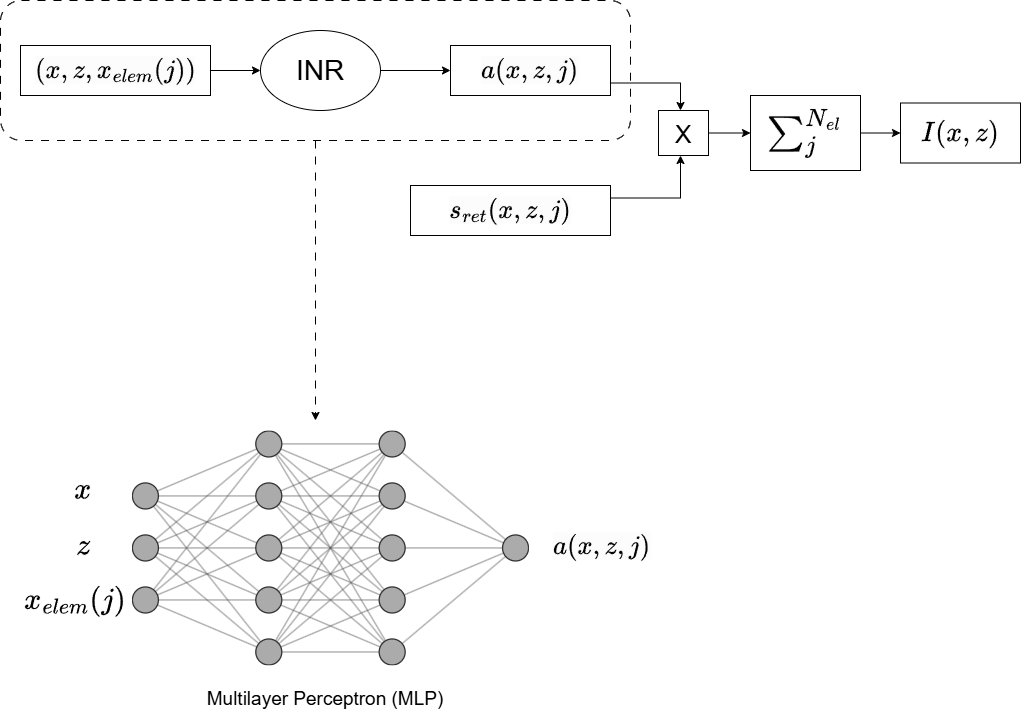
\includegraphics[width=0.8\textwidth]{tfm_esquema_inr.png}
  \caption{Esquema de generación de apodizaciones mediante una INR y su aplicación a DAS. La red calcula el peso $a(x,z,j)$ a partir de la geometría del píxel y del elemento $j$; este peso multiplica la señal retardada $s_{ret}(x,z,j)$ antes de la suma sobre los elementos. El esquema inferior ilustra la estructura de una MLP. Figura reproducida del TFM~\cite{CosarinskyTFM2026}.}
  \label{fig:tfm_arquitectura}
\end{figure}

El entrenamiento se realizó con datos simulados mediante PyMUST~\cite{Bernardino2024PyMUST} para una sonda lineal de 128 elementos. Se generaron 100 escenarios con 100 reflectores puntuales cada uno y 11 emisiones de ondas planas entre $-5^\circ$ y $5^\circ$, reservando el 20\% de los escenarios para validación. Como objetivo de aprendizaje se construyó una referencia sintética multiplicando la imagen DAS con apodización uniforme por una máscara gaussiana centrada en las posiciones conocidas de los reflectores. De este modo se buscó conservar sus respuestas y atenuar el fondo y los lóbulos laterales. La función de pérdida combinó un error absoluto medio ponderado, con mayor peso en las zonas de los reflectores, y una regularización que penaliza apodizaciones de amplitud media demasiado baja para evitar la supresión indiscriminada de señal. Se utilizó el optimizador Adam durante 40 épocas.

La apodización aprendida presentó una apertura que aumenta con la profundidad, con una distribución semejante a una ventana de Hanning dinámica con $F_{\#}=0.5$, aunque esta forma no se impuso como objetivo del entrenamiento de imagen. La evaluación se realizó sobre una grilla de reflectores, comparando la INR con apodizaciones uniforme, rectangular de apertura dinámica (\textit{boxcar}) y Hanning. La Figura~\ref{fig:tfm_imagenes} muestra las imágenes obtenidas y la Figura~\ref{fig:tfm_metricas} resume la anchura de las respuestas laterales (FWHM) y la relación señal-ruido (SNR), según las definiciones empleadas en el TFM.

\begin{figure}[H]
  \centering
  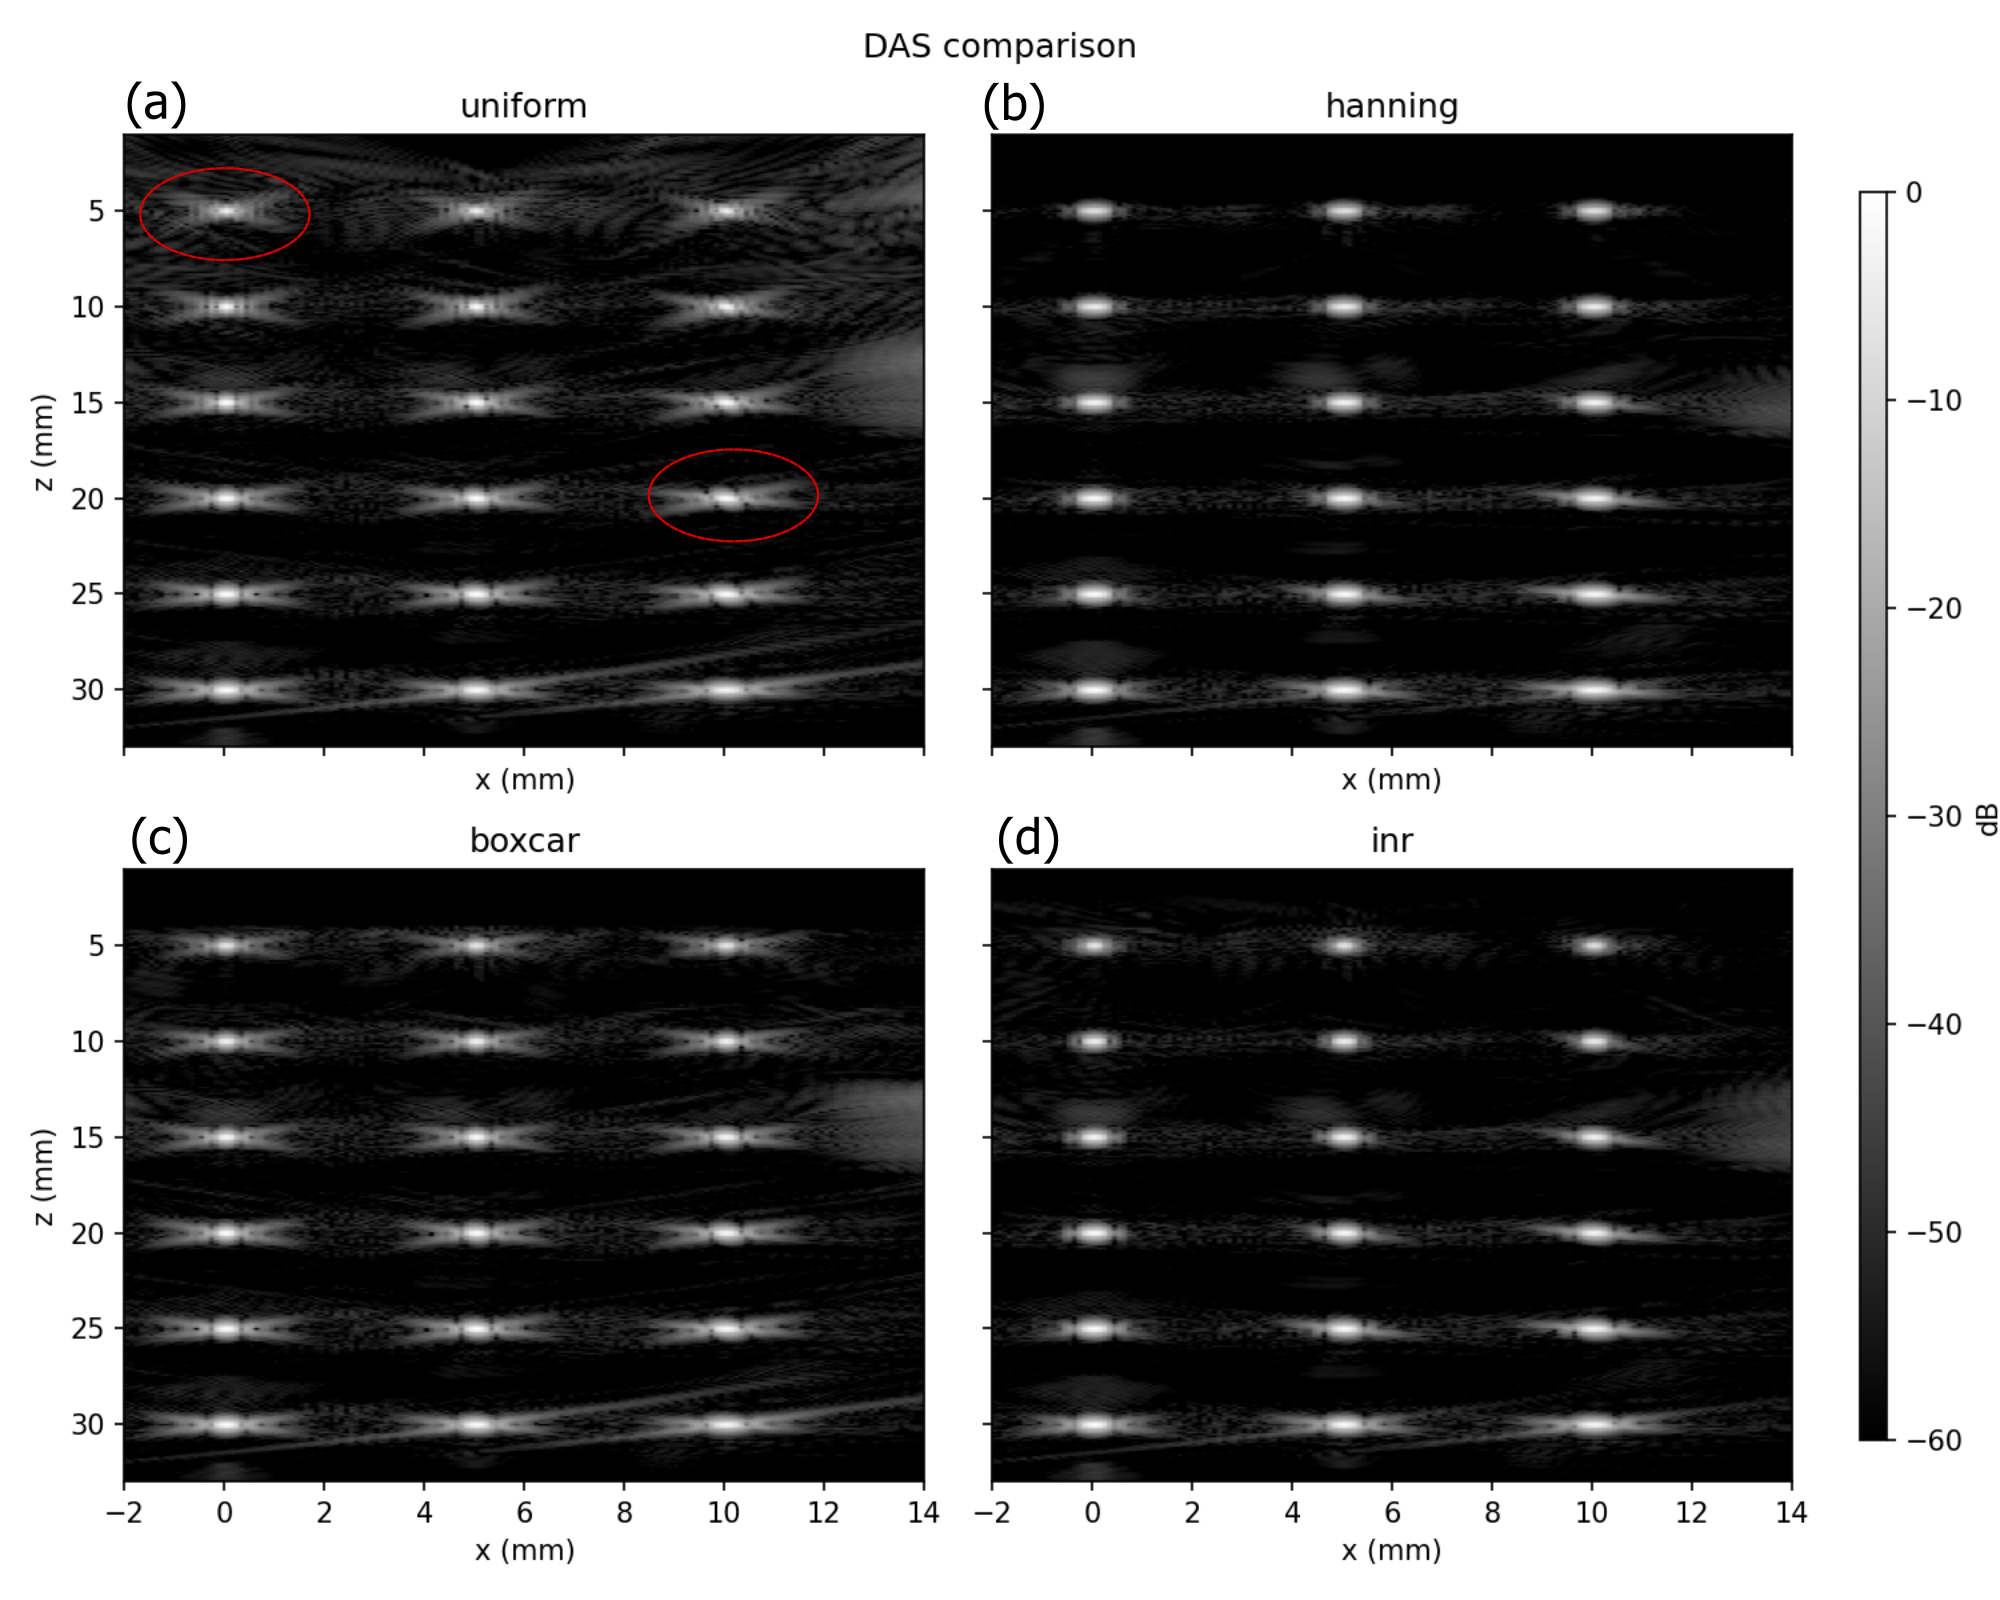
\includegraphics[width=0.95\textwidth]{tfm_comparacion_imagenes.png}
  \caption{Imágenes DAS de una grilla de reflectores simulados con apodización (a) uniforme, (b) Hanning dinámica, (c) rectangular de apertura dinámica y (d) aprendida mediante INR. La escala de visualización está indicada en dB. Figura reproducida del TFM~\cite{CosarinskyTFM2026}.}
  \label{fig:tfm_imagenes}
\end{figure}

En esta evaluación, la INR obtuvo respuestas laterales más estrechas que Hanning en los reflectores analizados, con una diferencia mayor cerca de la sonda. La SNR fue próxima a la de Hanning, aunque algo inferior en buena parte de las posiciones más profundas. Frente a la apodización uniforme, el resultado mantuvo un compromiso entre anchura de la respuesta y supresión del fondo: la mejora de SNR estuvo acompañada de respuestas generalmente más anchas. Por tanto, el resultado principal fue la capacidad de aprender una distribución espacial de pesos con un equilibrio entre ambas propiedades, dentro del conformador DAS.

\begin{figure}[H]
  \centering
  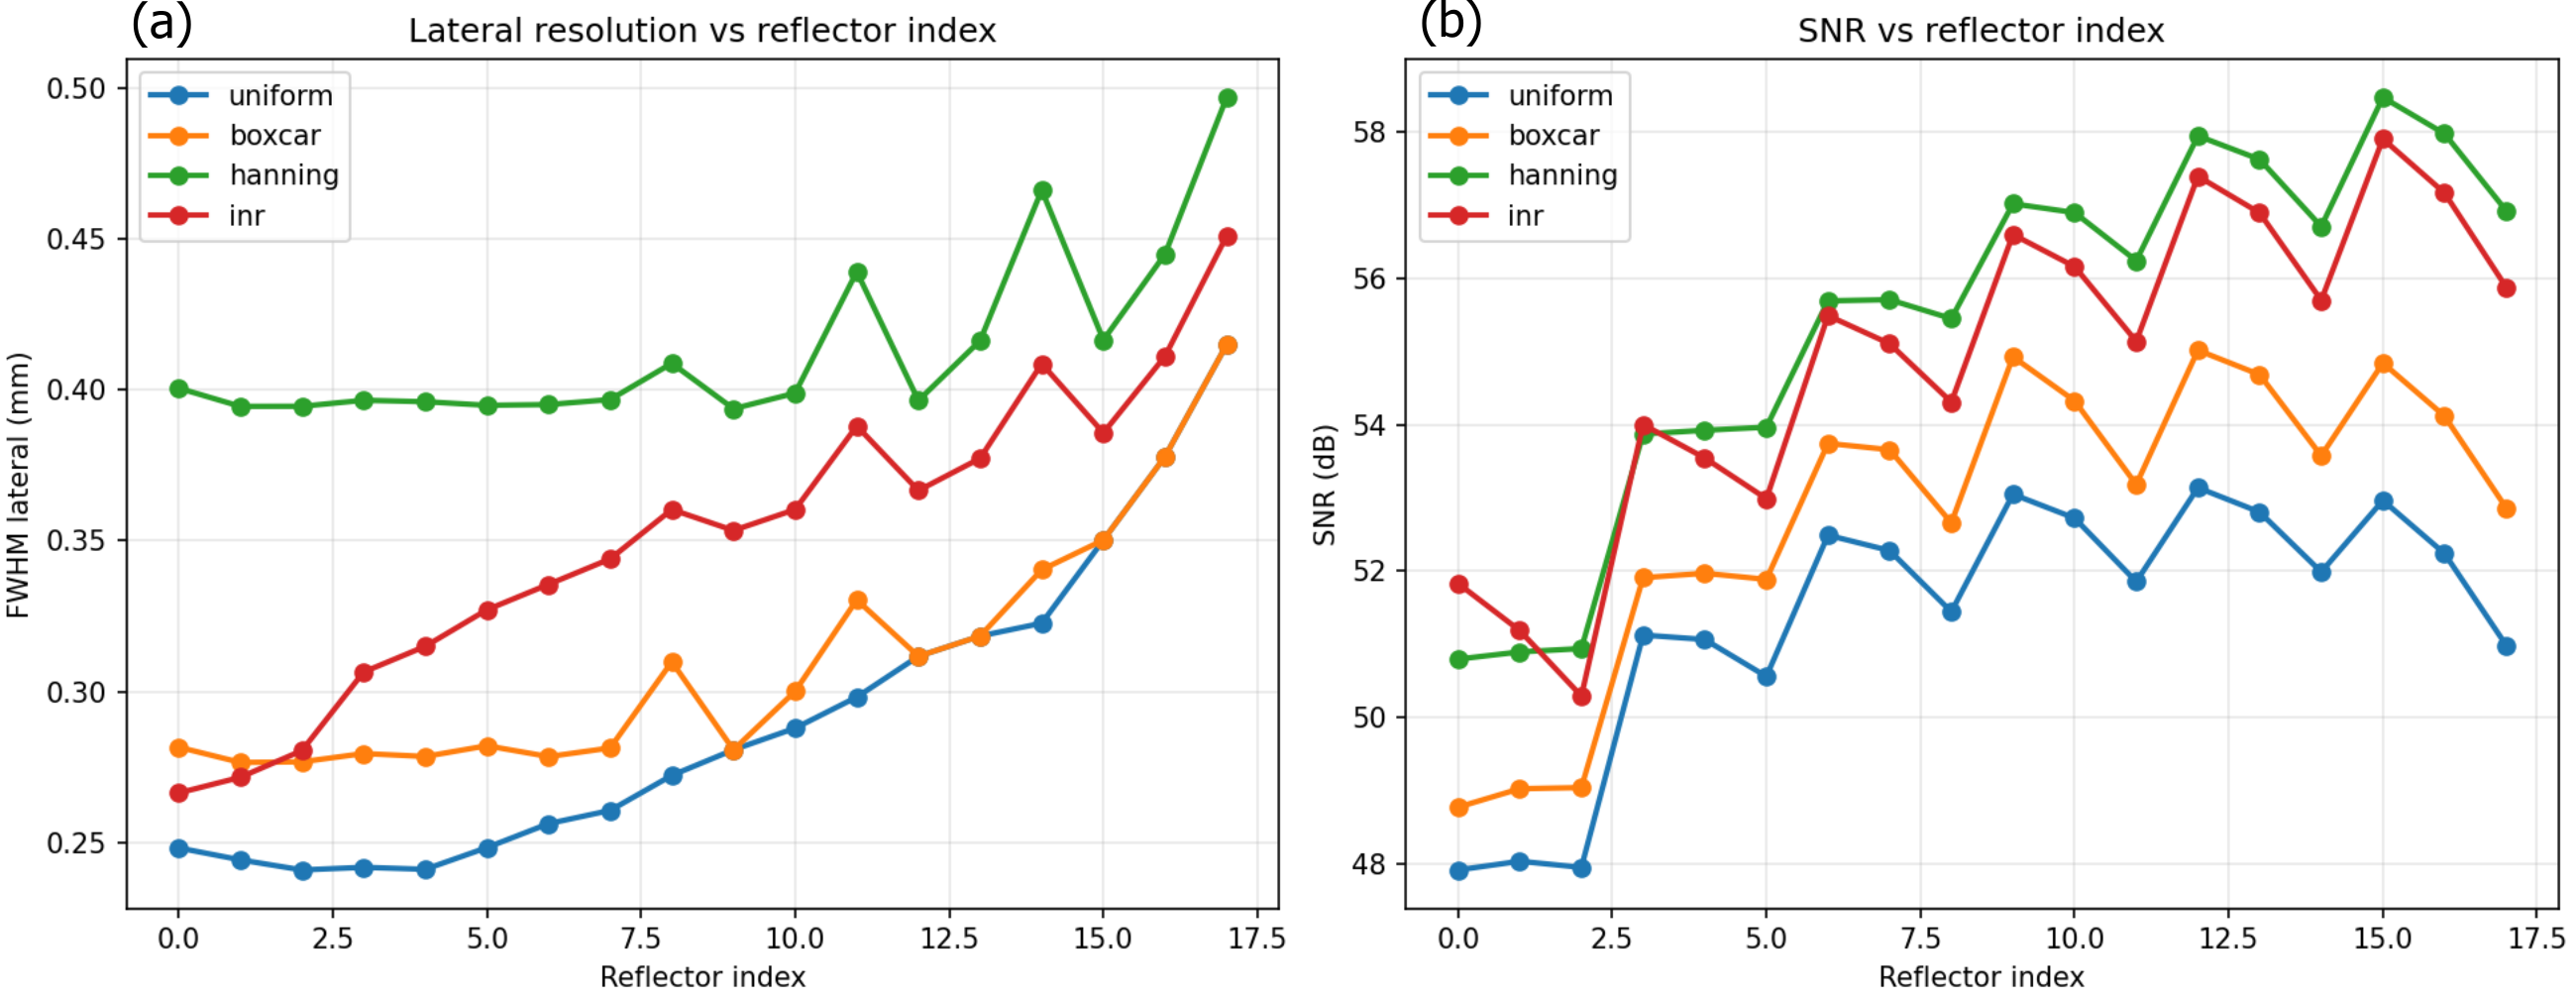
\includegraphics[width=\textwidth]{tfm_comparacion_metricas.png}
  \caption{Evaluación por reflector de las apodizaciones de referencia y de la INR: (a) anchura lateral FWHM y (b) SNR. Los resultados corresponden a la grilla simulada mostrada en la Figura~\ref{fig:tfm_imagenes}. Figura reproducida del TFM~\cite{CosarinskyTFM2026}.}
  \label{fig:tfm_metricas}
\end{figure}

El alcance del TFM fue una prueba de concepto en simulación con reflectores puntuales en un medio homogéneo. La validación experimental quedó fuera de este trabajo. La formulación de una única apodización real y positiva proporcionó la base para la extensión posterior a múltiples apodizaciones y su combinación neuronal, descrita en la siguiente subsección. La memoria completa del TFM se adjunta en el Anexo~\ref{anexo:tfm}.
\FloatBarrier


\subsection{Diseño y combinación de múltiples apodizaciones mediante redes neuronales}\label{sec:tecniacustica}
\begingroup
\emergencystretch=2em
Esta subsección sintetiza la continuación del TFM presentada en Tecniacústica 2026~\cite{CosarinskyTecniacustica2026}. El artículo completo, con los detalles del método y de su evaluación, se incluye en el Anexo~\ref{anexo:tecniacustica}.

El trabajo amplió el diseño de una única apodización a un conjunto de apodizaciones aprendidas y una regla de combinación también neuronal, tomando como referencia la estructura de NSI. La motivación fue la pérdida de apertura efectiva que se produce cerca de los extremos del array cuando, para conservar el equilibrio de los pesos de NSI, la subapertura se reduce de forma simétrica. Se buscó explorar si el aprendizaje conjunto de los pesos de recepción y de la combinación de imágenes permitía mejorar la respuesta en esas regiones.

La arquitectura incorpora dos redes. La primera es una INR que genera $M$ funciones de apodización $a_m(x,z,x_{elem};\omega)$ a partir de las coordenadas del píxel y del elemento receptor. Cada función pondera las señales retardadas para producir una imagen DAS:
\begin{equation}
  I_m(x,z)=\sum_j a_m(x,z,x_{elem}(j);\omega)\,s_{ret}(x,z,j),
  \qquad m=1,\ldots,M.
  \label{eq:mixer_imagenes}
\end{equation}
Las envolventes de estas imágenes se combinan píxel a píxel mediante una segunda MLP, denominada \textit{mixer}:
\begin{equation}
  I_{\mathrm{final}}(x,z)=g_{\phi}\left(|I_1(x,z)|,\ldots,|I_M(x,z)|\right),
  \label{eq:mixer_combinacion}
\end{equation}
donde $\omega$ y $\phi$ representan los parámetros entrenables de ambas redes. De este modo, se aprende tanto la generación de las imágenes intermedias como su combinación no lineal. Una vez entrenada la INR, las apodizaciones dependen de la geometría y se aplican a las distintas adquisiciones. El \textit{mixer} se mantuvo pequeño para limitar el coste adicional de cálculo. La Figura~\ref{fig:tecni_arquitectura} resume el proceso.

\begin{figure}[H]
  \centering
  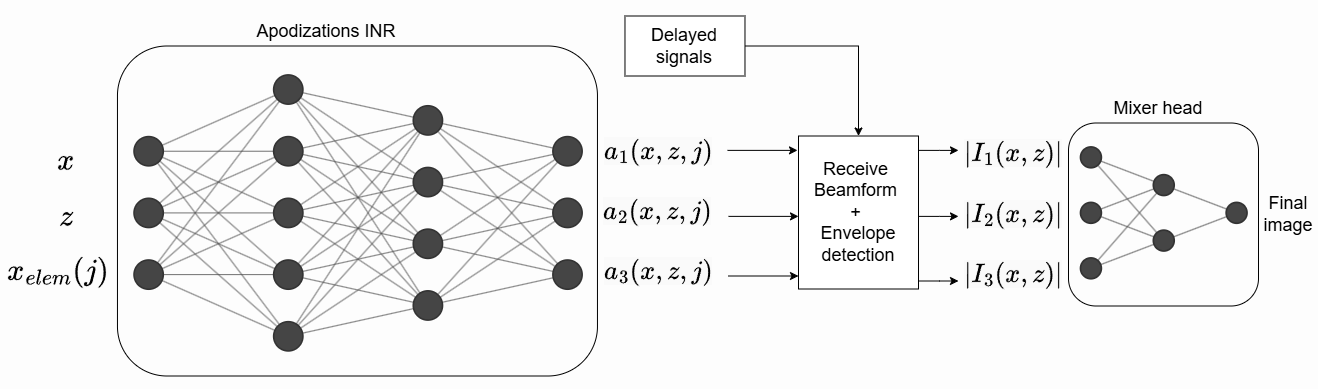
\includegraphics[width=\textwidth]{tecni_arquitectura.png}
  \caption{Arquitectura para generar múltiples apodizaciones mediante una INR y combinar las envolventes de las imágenes resultantes con un \textit{mixer}. El esquema ilustra tres canales de apodización; la configuración seleccionada para los resultados del artículo utilizó dos. Figura reproducida del trabajo de Tecniacústica~\cite{CosarinskyTecniacustica2026}.}
  \label{fig:tecni_arquitectura}
\end{figure}

El entrenamiento utilizó señales simuladas con PyMUST~\cite{Bernardino2024PyMUST}, en un medio homogéneo con reflectores puntuales y con la configuración de sonda de PICMUS~\cite{liebgott2016picmus}. Se simularon once ondas planas entre $-5^\circ$ y $5^\circ$. Como en el TFM, las referencias de entrenamiento se construyeron multiplicando una reconstrucción DAS por una máscara gaussiana centrada en los reflectores. La optimización minimizó el error absoluto medio respecto a estas referencias. Además, cada apodización aprendida se multiplicó por una ventana de Hanning de apertura dinámica con $F_{\#}=1$, para restringir los pesos hacia los extremos de la apertura. Entre las configuraciones ensayadas se seleccionó una INR con tres capas ocultas de 16, 8 y 4 neuronas y dos canales de apodización, junto con un \textit{mixer} de dos capas ocultas.

La evaluación comparó el método con DAS de apodización Hanning dinámica y con NSI, utilizando una grilla simulada de reflectores y una adquisición experimental de un fantoma PICMUS~\cite{liebgott2016picmus}. En simulación, el método mejoró la resolución lateral respecto a DAS, aunque NSI mantuvo un mejor comportamiento en la mayor parte de la imagen. La mejora más relevante se localizó en un reflector próximo al extremo lateral del array, donde el método aprendido obtuvo una respuesta más estrecha que NSI. Asimismo, en la columna de reflectores situada en $x=18$~mm, próxima al borde del array en $x=19.5$~mm, NSI presentó una caída de amplitud al aumentar la profundidad que no se observó con el método propuesto ni con DAS (Figura~\ref{fig:tecni_simulacion}).

\begin{figure}[H]
  \centering
  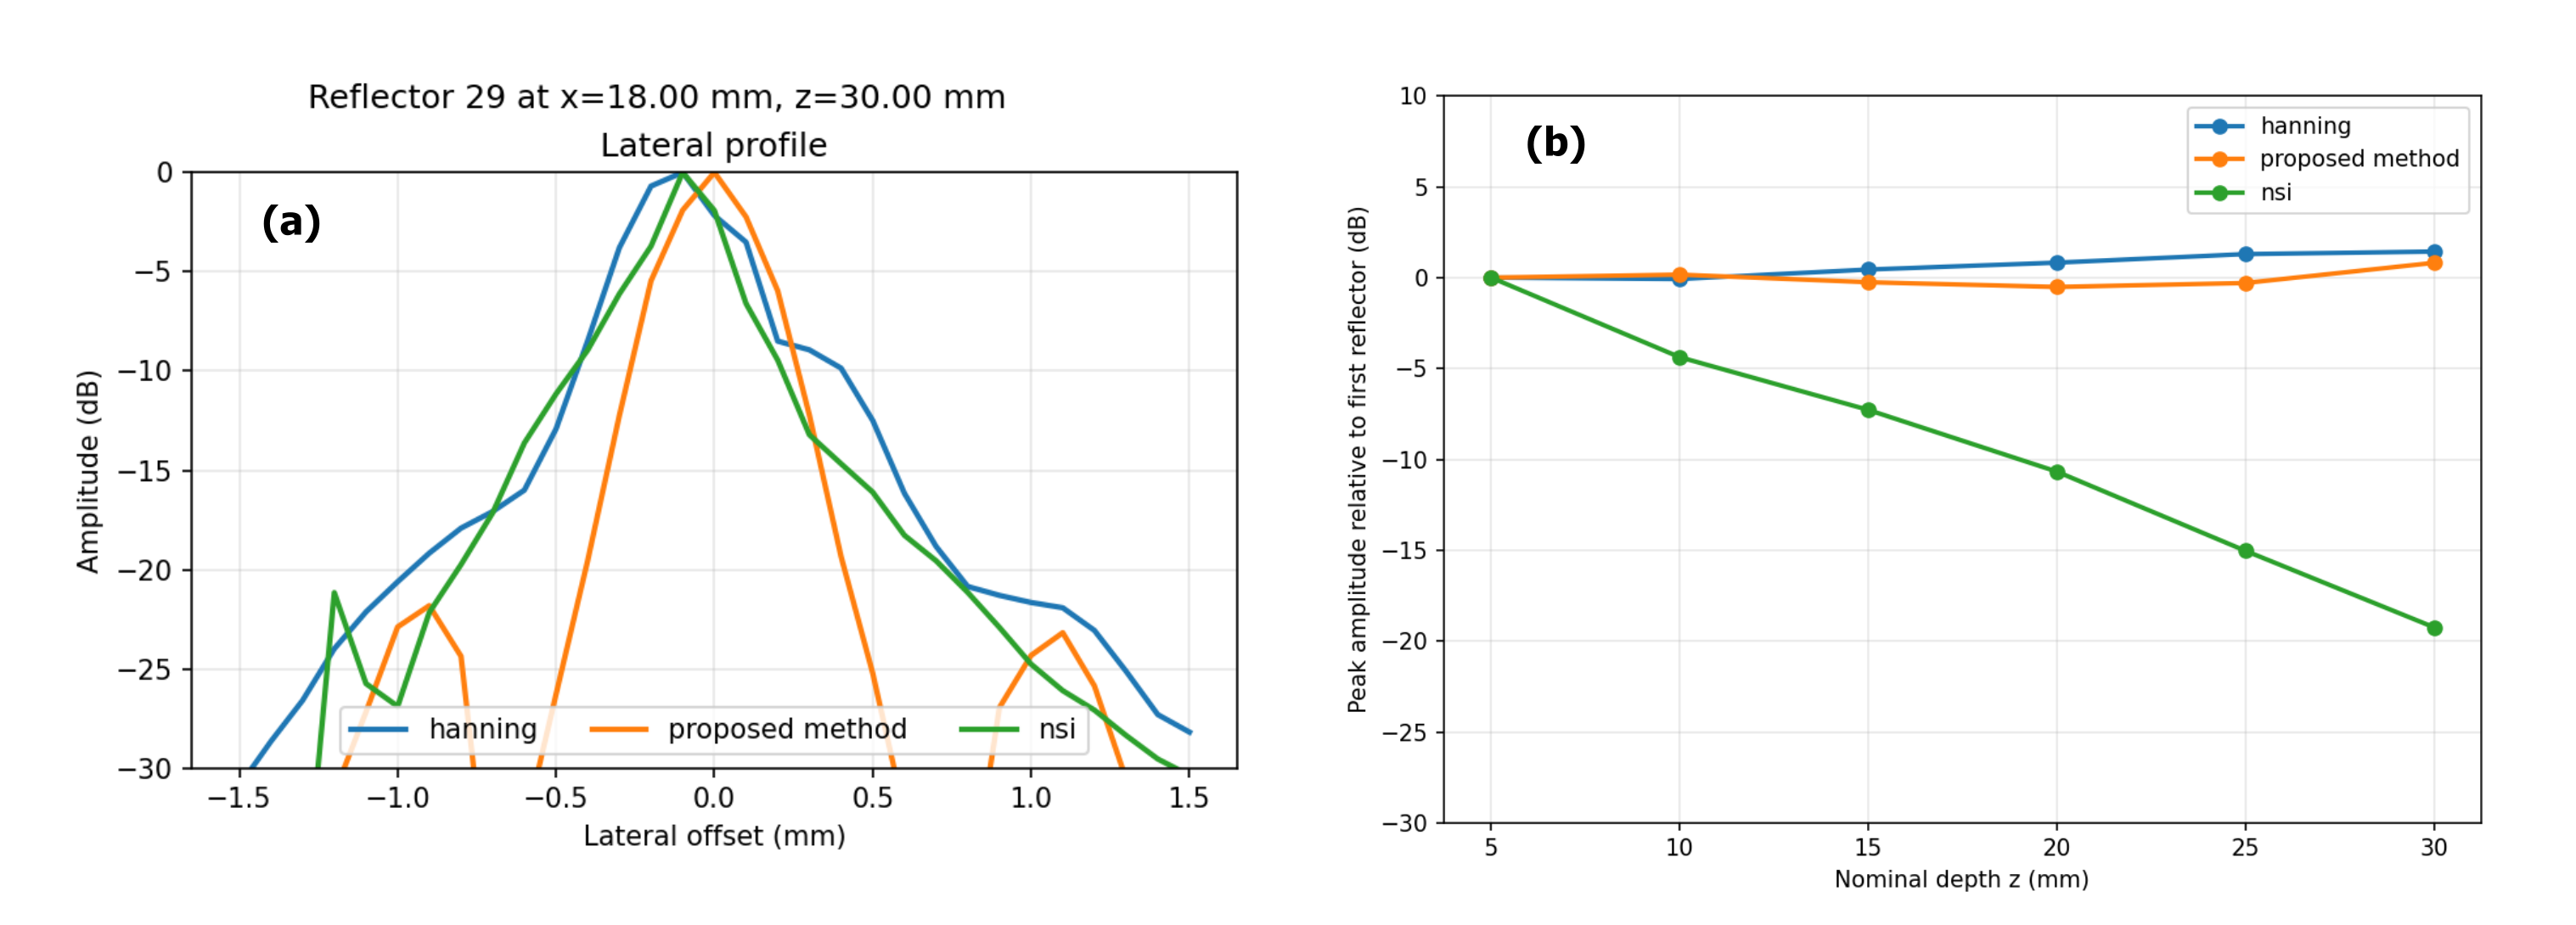
\includegraphics[width=\textwidth]{tecni_resultados_borde.png}
  \caption{Resultados simulados cerca del borde lateral del array: (a) perfil de un reflector situado en $x=18$~mm y $z=30$~mm; (b) amplitudes máximas de los reflectores de esa columna en función de la profundidad, relativas al primer reflector. Se comparan DAS con Hanning, NSI y el método aprendido. Figura reproducida del trabajo de Tecniacústica~\cite{CosarinskyTecniacustica2026}.}
  \label{fig:tecni_simulacion}
\end{figure}

En la adquisición experimental, NSI ofreció la mejor resolución lateral global, mientras que la reconstrucción aprendida fue, en conjunto, comparable a DAS. Los perfiles de reflectores seleccionados cerca del borde mostraron mejoras locales de resolución, menos pronunciadas que en simulación (Figura~\ref{fig:tecni_picmus}). Esta evaluación permitió comprobar la aplicación del modelo entrenado con simulaciones a datos experimentales, manteniendo el carácter preliminar de los resultados.

\begin{figure}[H]
  \centering
  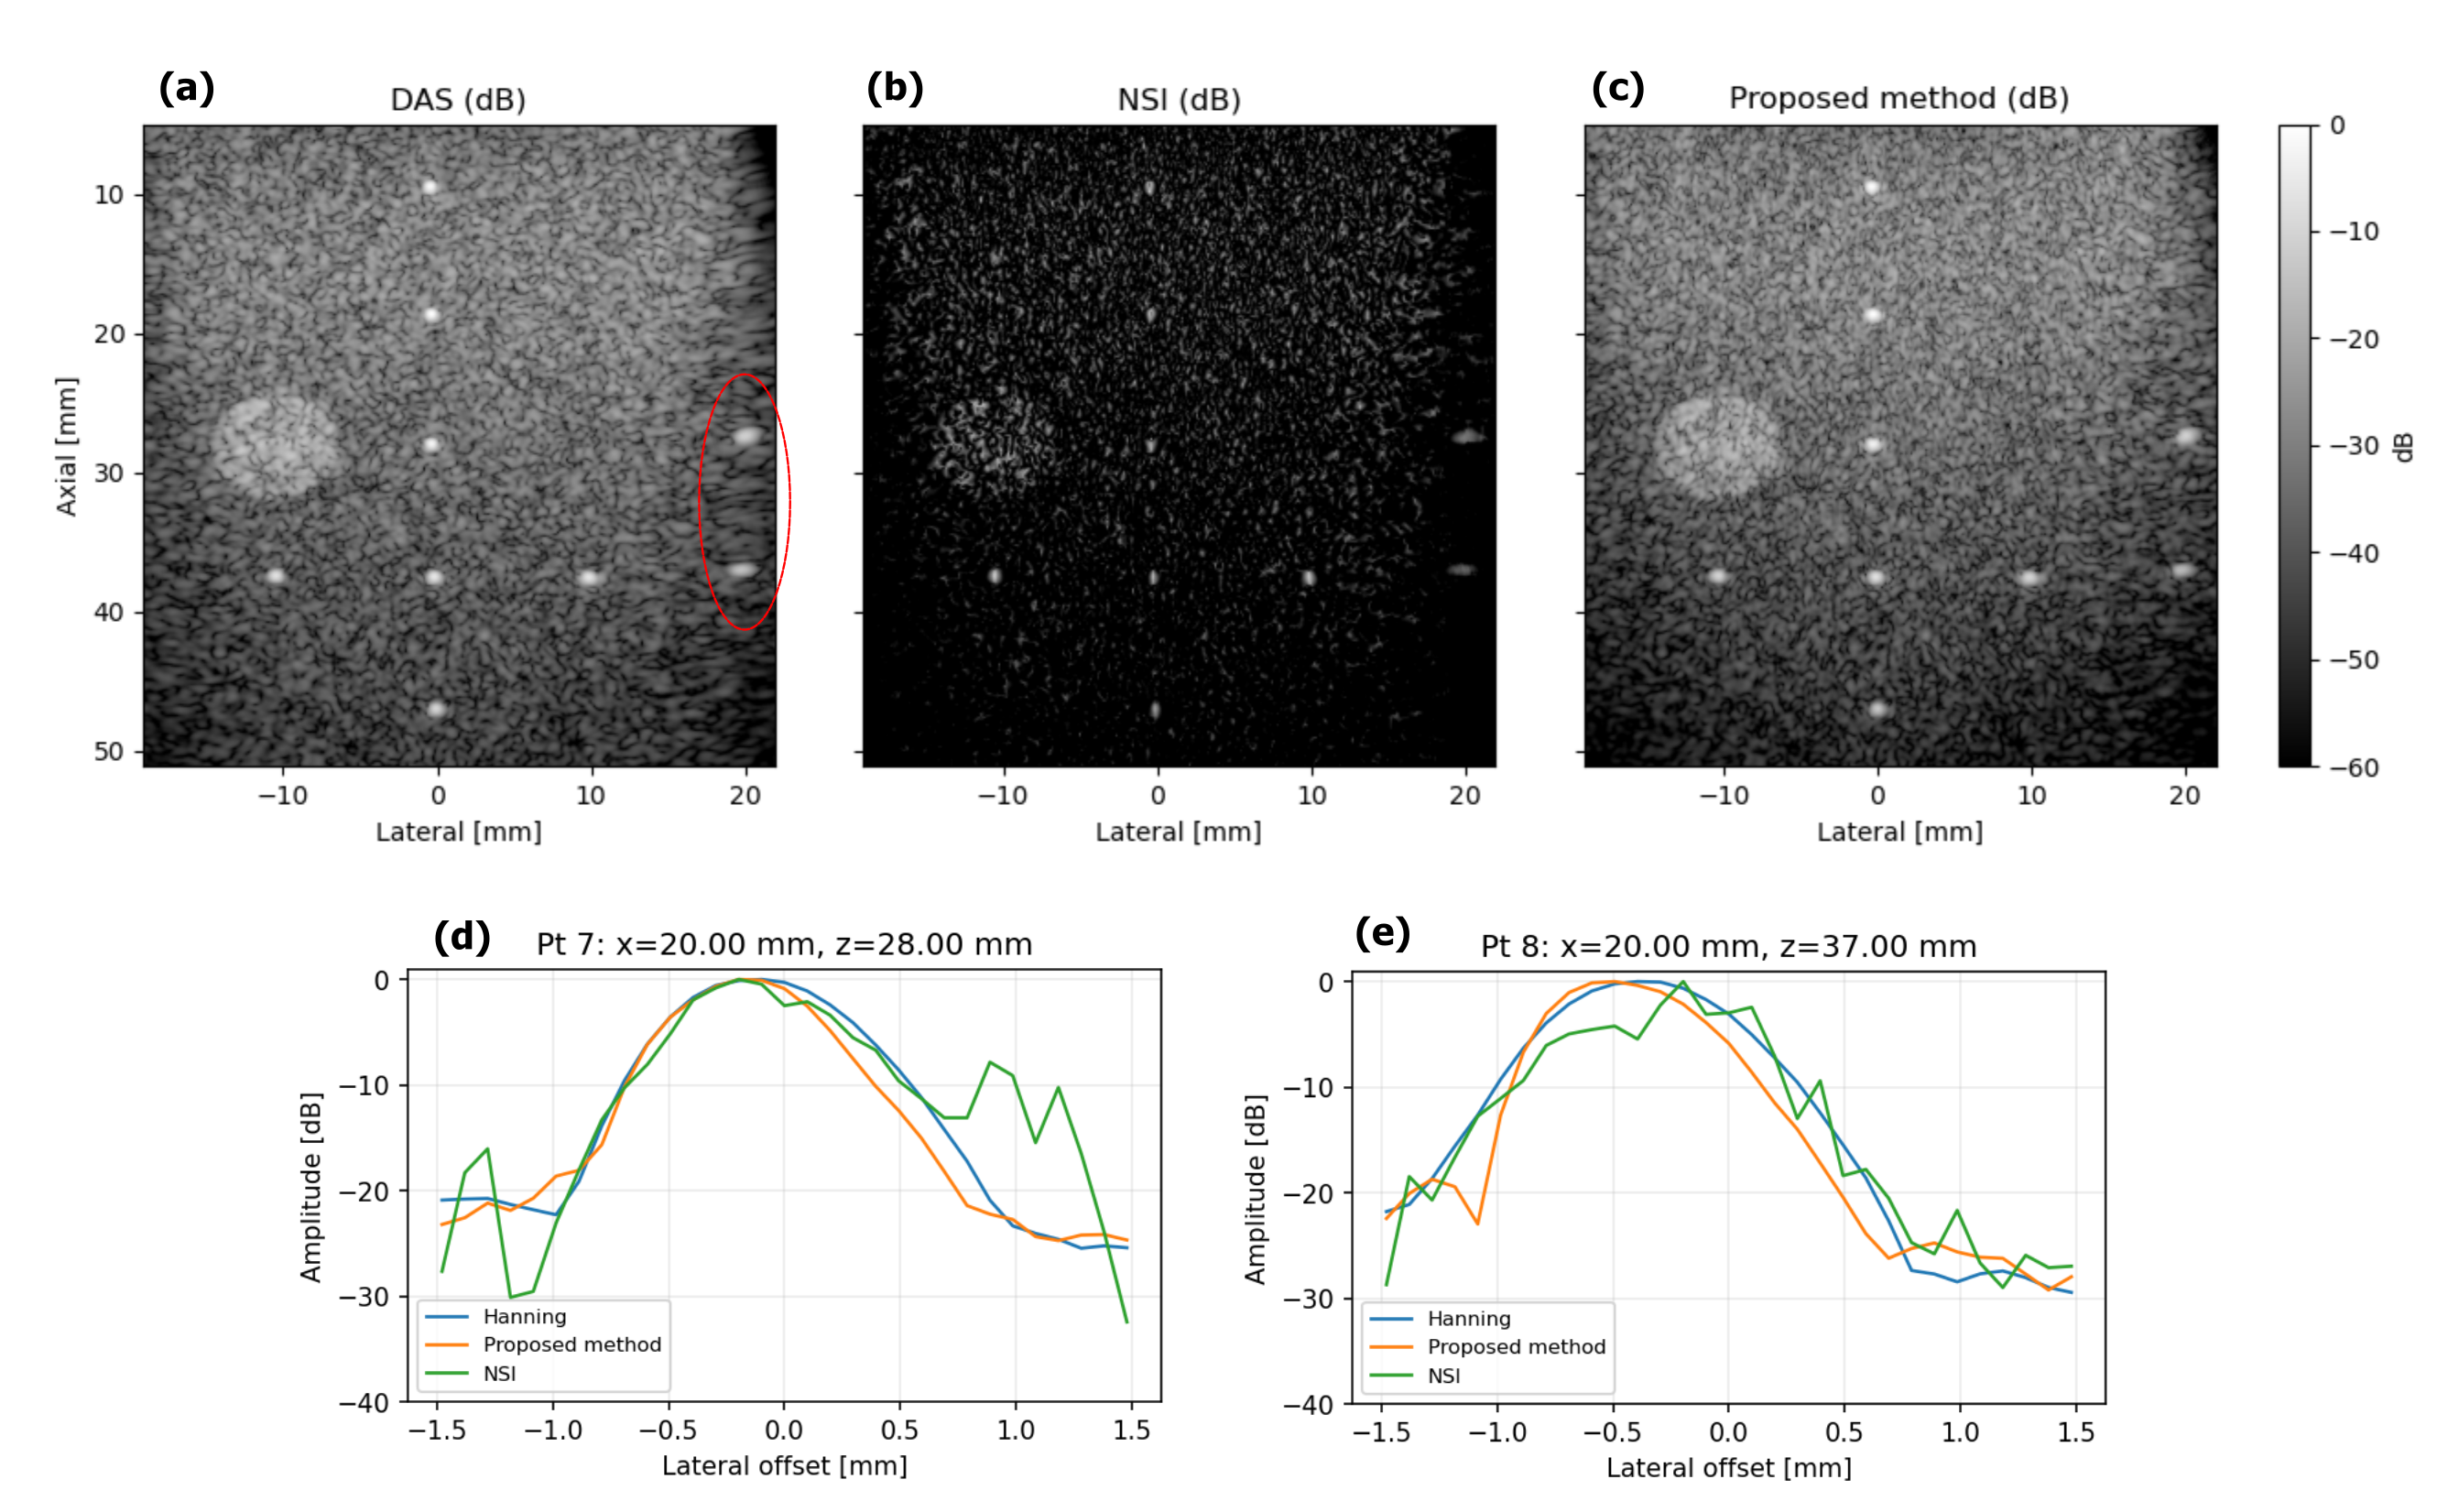
\includegraphics[width=\textwidth]{tecni_resultados_picmus.png}
  \caption{Evaluación experimental en un fantoma PICMUS~\cite{liebgott2016picmus}: imágenes obtenidas con (a) DAS, (b) NSI y (c) el método aprendido; (d, e) perfiles laterales de dos reflectores próximos al borde, en $x=20$~mm. Figura reproducida del trabajo de Tecniacústica~\cite{CosarinskyTecniacustica2026}.}
  \label{fig:tecni_picmus}
\end{figure}

En conjunto, el trabajo estableció un esquema de aprendizaje de múltiples apodizaciones y de su combinación, con indicios de mejora en regiones donde la restricción de simetría limita la apertura de NSI. Las ventajas observadas fueron locales y la configuración evaluada no alcanzó el rendimiento global de NSI. Estos resultados motivan seguir investigando cómo influyen el número de apodizaciones, la arquitectura de las redes y el objetivo de entrenamiento en la calidad de las imágenes obtenidas.
\FloatBarrier
\endgroup

\section{Estancia en la UCM e inicio de la línea de guiado de ecocardiografía}\label{sec:ucm}
% Extension orientativa: 1--1.5 paginas.

\subsection{Marco y objetivos de la estancia}
\pendiente{Presentar la estancia bajo la supervisión de Joaquín López Herraiz, en el Departamento de Estructura de la Materia, Física Térmica y Electrónica de la UCM. El periodo previsto en la carta de invitación es del 16 de septiembre al 11 de diciembre de 2026; actualizar con las fechas efectivas al cierre.}

\pendiente{Introducir brevemente el objetivo de investigar métodos de IA para el guiado de ecocardiografía transtorácica (TTE) y su relación con las competencias desarrolladas en el proyecto.}

\subsection{Actividades iniciales y estado de la línea}
\pendiente{Documentar únicamente las actividades efectivamente realizadas y el estado inicial del trabajo al cierre de la memoria. Añadir los próximos pasos inmediatos sin presentar como resultados las tareas previstas.}

\section{Formación y difusión de resultados}\label{sec:formacion}
% Extension orientativa: 1--2 paginas.

\subsection{Formación y competencias adquiridas}
\pendiente{Resumir la finalización del Máster de Formación Permanente en Inteligencia Artificial Aplicada de la Universidad Europea y la realización del TFM. La ficha de actividad de 2026 recoge los módulos 5 a 10 con 36 ECTS; completar fechas y otras actividades con sus justificantes, evitando duplicidades entre anualidades.}

\begin{table}[htbp]
  \centering
  \small
  \begin{tabularx}{\textwidth}{@{}Xll@{}}
    \toprule
    \textbf{Actividad} & \textbf{Periodo} & \textbf{ECTS / horas} \\
    \midrule
    Máster en IA Aplicada, módulos 5 a 10 (incluido el TFM) & Ene.--may. 2026 & 36 ECTS \\
    \bottomrule
  \end{tabularx}
  \caption{Actividades formativas correspondientes a 2026. Completar con las actividades acreditadas del periodo.}
  \label{tab:formacion}
\end{table}

\pendiente{Relacionar brevemente la formación con las competencias aplicadas: simulación, aprendizaje supervisado, diseño y evaluación de modelos y procesamiento de imagen ultrasónica.}

\subsection{Difusión y colaboraciones}
\pendiente{Documentar la contribución presentada en Tecniacústica 2026, su relación con el TFM y otras actividades acreditadas de difusión o colaboración realizadas durante el año.}

\section{Balance del año y continuidad}\label{sec:conclusiones}
% Extension orientativa: una pagina.
\pendiente{Sintetizar los desarrollos realizados, la aplicación de la formación en IA a la investigación en ultrasonidos y el inicio de la colaboración con la UCM. Cerrar con una descripción breve de la continuidad prevista de ambas líneas.}

\FloatBarrier
{\raggedright\printbibliography[heading=bibintoc,title={Referencias}]\par}


\appendix
\clearpage
\section{Memoria completa del Trabajo de Fin de Máster}\label{anexo:tfm}
%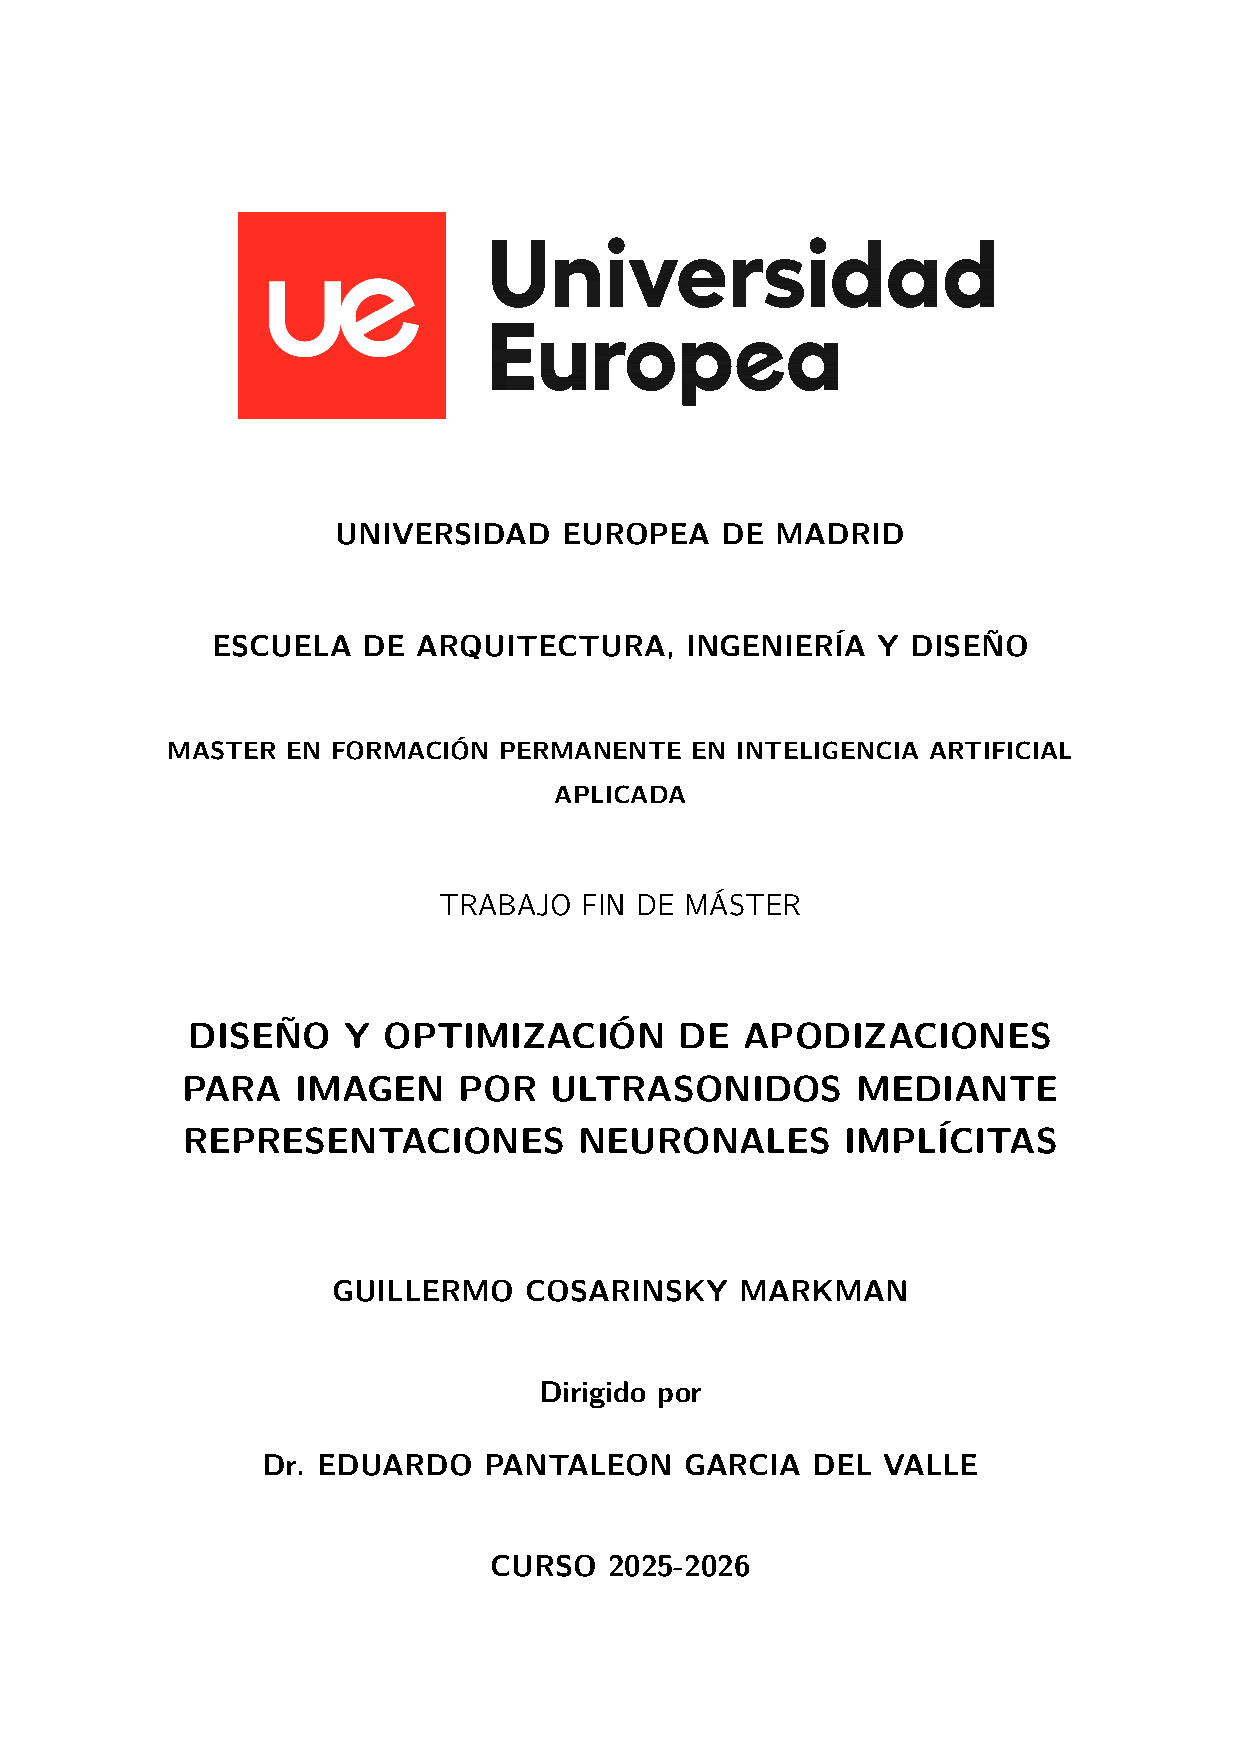
\includepdf[pages=-]{apendices/TFM_cosarinsky_main.pdf}

\clearpage
\section{Artículo presentado en Tecniacústica 2026}\label{anexo:tecniacustica}
%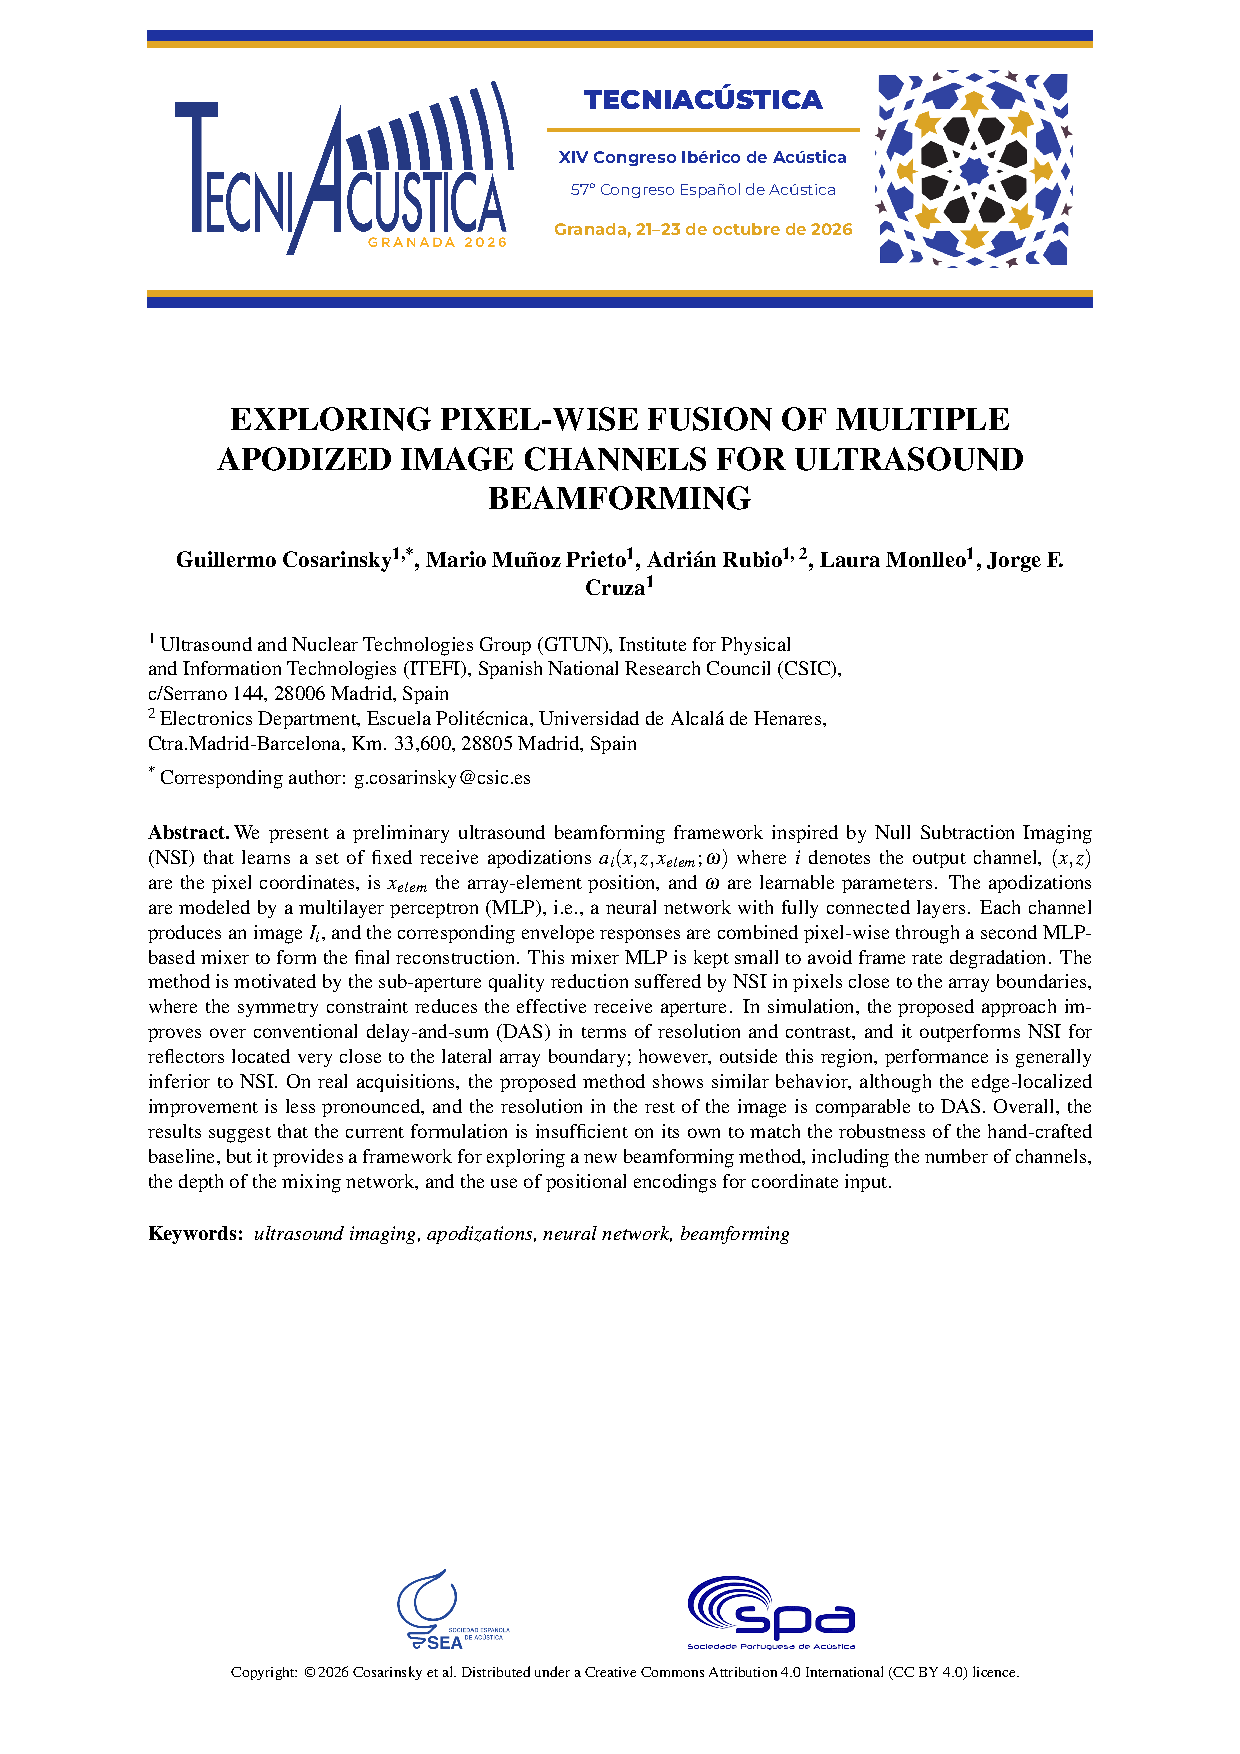
\includepdf[pages=-]{apendices/cosarinsky_tecniacustica2026.pdf}

\clearpage
\section{Justificantes de formación, estancia y difusión}\label{anexo:justificantes}
\pendiente{Incorporar únicamente los justificantes que se requieran para la memoria.}
% Ejemplo: \includepdf[pages=-]{apendices/justificante.pdf}

\end{document}
